


A \emph{Transaction Processing System (TPS)} runs atop an underlying data store 
(e.g., HBase) and 
allows users to bundle multiple data store operations into a single atomic transaction. 
The TPS architecture is depicted in Figure~\ref{fig:components}.
Section~\ref{ssec:data-model} describes the data model and API of the underlying data store, and  Section~\ref{ssec:transactions}
defines transaction semantics provided by the TPS. 

\begin{figure}
\centerline{
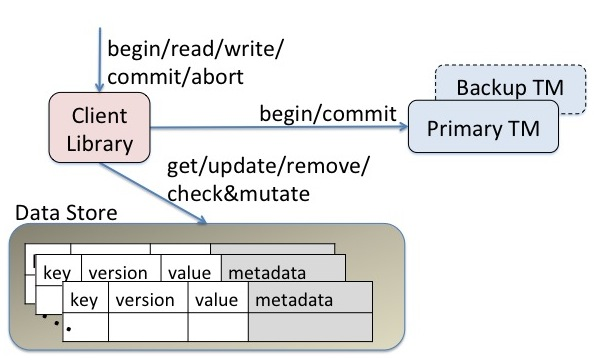
\includegraphics[width=0.45\textwidth]{FragolaComponents.jpg}
}
\caption{Transaction processing architecture: A client library exposes an  API for  executing transactions of data store operations. 
A centralized Transaction Manager handles transaction begin and commit requests, while data is written directly to the underlying data store.
The TM has a backup for high availability.}
\label{fig:components}
\end{figure}

\subsection{Data store}
\label{ssec:data-model}

The  data store holds  \emph{objects} (often referred to as \emph{rows}) identified by unique \emph{keys}.
Each row can consist of multiple \emph{fields}, representing different \emph{columns}. 
We consider multi-versioned objects, where object values are associated with \emph{version numbers}, and
multiple versions associated with the same key may co-exist.
\remove{
Thus, at any given time, an object holds a tuple \tuple{key,\tuple{version,value}+}, where value
can be structured to consist of multiple columns.
}
We further assume that a write operation can specify the version number it writes to.
%monotonically increasing ??
%\paragraph{API} 
The  data store provides the following API:
\begin{description}
\item [\code{get(key, version)}] --  returns the requested version of key.
%if no version is provided, returns the latest; 
%if no field is provided returns the entire record. 
%\item 
The API further allows traversing (reading) earlier versions of the same key.
% in descending order.
\item [\code{update(key, version, fields, values)}] -- 
creates or updates an object, setting the specified fields to the specified values. 
If the version already exists, its value is updated; otherwise, a new version is added. 
\remove{The data store may buffer the write in memory until an ensuing flush. }
\item [\code{remove(key, version)}] -- removes an object with the given key and version.
\item [\code{check\&mutate(key, version, field, old, new)}] -- checks the record associated with key and version. 
If field holds old, replace it with new   and return true; otherwise return false.
\remove{ \item [\code{flush}] -- persists all previous updates to disk.}
%data stores often provide means to atomically read and update a single object, e.g., HBase exports check\&mutate operations, which are 
%internally implemented using a per-row RW lock.
%, whereas BigTable supports row transactions. 
%We will extend this capability below in order to implement certain atomic operations at the data store level.
\end{description}

A separate process performs garbage collection of obsolete versions.

\subsection{Transaction semantics} \label{ssec:transactions}

TPSs provide \emph{begin} and \emph{commit} APIs for delineating transactions: 
a \emph{transaction} is a sequence of \emph{read} and \emph{write} operations on different objects 
that occur between begin and commit. Note that transactional reads and writes are implemented using the 
datastore's get and put operations.
Two transactions are said to be \emph{concurrent} if 
their executions overlap, i.e., one of them begins between the begin time and commit time of the other;
otherwise, we say that they are \emph{non-overlapping}.

A TPS  ensures the ACID properties for transactions:
\emph{atomicity} (all-or-nothing), \emph{consistency} (preserving each object's semantics), 
\emph{isolation} (in that concurrent transactions do not see each other's partial updates), and 
\emph{durability} (whereby updates survive crashes).

Different isolation levels can be considered for the third property. We consider a variant of 
\emph{snapshot isolation (SI)}~\cite{DBLP:conf/sigmod/BerensonBGMOO95} that, similarly to \emph{generalized snapshot isolation}~\cite{DBLP:conf/srds/ElniketyZP05}, relaxes  the real-time order requirement. 
Nevertheless, our implementation only relaxes the ordering of fast path  transactions (described in Section~\ref{sec:alg}) 
relative to regular ones (that do not use the fast path); regular transactions continue to satisfy SI amongst themselves. 
Moreover, \sysll, without the fast path, satisfies SI as Omid does.

Our relaxed correctness condition satisfies the key ``snapshot'' property of SI, which ensures that a transaction reading from the  database
does not see a mix old and new values. For example, if a transaction updates the values of two stocks, 
then no other transaction may observe the old value of one of these stocks and the new value of the other.
However, it relaxes the real-time order guarantee of SI by allowing (fast-path) transactions to take effect `in the past'.  
 \remove{ % Idit: removed the example and figure to save space
Similarly, a regular transaction overlapping
two fast path ones may observe an update of the second and miss an update by the first,  as illustrated in 

Figure~\ref{fig:ltx-rt}, shows an example where fast path transaction FP2 is ordered `in the past'.
%Yet we do enforce real-time order on regular transactions as well as on all updates of the same key.

\begin{figure}[ht]
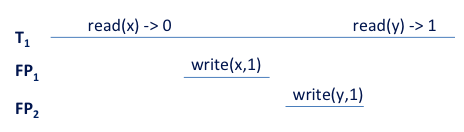
\includegraphics[width=\columnwidth]{figs/FP-semantics}
\caption{Possible violation of real-time order among fast path transactions. Regular transaction $T_1$
reads $x$ before it is updated by fast path transaction $FP_1$ and reads $y$ after it is updated by fast path transaction $FP_2$ even 
though $FP_2$ occurs after $FP_1$. 
%$T1$'s global version is $10$, and its skips the local version clocks of the regions holding $x$ and $y$ to $10$ when reading from them.
}
\label{fig:ltx-rt}
\end{figure}
} % remove
Specifically, %our correctness condition stipulates that
the system enforces a total order ${\cal T}$ on all committed transactions, so that
\begin{enumerate}
    \setlength{\itemsep}{0pt}
    \setlength{\parskip}{0pt}
    \setlength{\parsep}{2pt}  
%\item
%regular transactions (though not FP ones) are ordered in ${\cal T}$  according to their commit times;
\item
non-overlapping transactions 
%(regular and FP) 
that update the same key occur in ${\cal T}$  in order of their commit times;
\item
each  transaction's read operations see a consistent snapshot of the database reflecting 
a prefix of  ${\cal T}$; 
%and  
%that includes at least all regular transactions committed prior to its start time; and 
\item
 a transaction commits only if none of the items it updates is modified by a transaction ordered in ${\cal T}$ after
 its snapshot time and before its commit time.
 \end{enumerate}

\remove{ % OLD SI definition - no relaxation of RTO
More precisely, 
SI enforces a total order on committed transactions according to their commit times so that 
\begin{enumerate}
    \setlength{\itemsep}{0pt}
    \setlength{\parskip}{0pt}
    \setlength{\parsep}{2pt}  
\item
each transaction's read operations see a consistent snapshot of the database reflecting write operations by
 exactly those transactions that committed prior to the transaction's start time; and 
\item
 a transaction commits only if none of the items it updates has been modified since that snapshot.
 \end{enumerate}
 } %Remove
 
Note that as with SI, two concurrent transactions conflict only if they both \emph{update} the same item.  
In contrast, under serializability, a transaction that updates an item also conflicts with transactions that \emph{read} that item. 
Snapshot isolation is thus amenable to implementations (using multi-versioning) that 
allow more concurrency than serializable ones, and hence scale better.
It is therefore provided by popular database technologies such as Oracle, PostgreSQL, and SQL Server,
and TPSs such as Percolator, Omid, Tephra, and  CockroachDB.

Following a commit call, the transaction may successfully \emph{commit}, whereby all of its operations take effect, 
or 
%in case of conflicts, (i.e., when two concurrent transactions attempt to update the same item), the transaction may
\emph{abort}, in which case none of its changes take effect. 



%An abort may also be initiated by the programmer, e.g., 
%on encountering an error. Applications typically retry a transaction upon  abort. 


%%%The data is \emph{partitioned} (or sharded), and each object belongs to one region. 
%%%%Global transactions may span multiple regions, and atomically commit or abort on all. 
%%%\emph{Local transactions} are ones that access a single region.
